%!TEX program=xelatex
\documentclass{article}

% Chinese font
\usepackage{xeCJK}
\usepackage{hyperref}

\setCJKmainfont{[kaiu.ttf]}
\setmainfont{[times new roman.ttf]}

\usepackage{colortbl}
\usepackage{xcolor}

\definecolor{LightGray}{gray}{0.8}
\newcolumntype{a}{>{\columncolor{LightGray}}c}
\newcolumntype{Y}{>{\centering\arraybackslash}X}

\usepackage{tabularx}
\usepackage{makecell}

\setcounter{section}{-1}
\renewcommand*\contentsname{目錄}

\usepackage{graphicx}

\graphicspath{{./img/}}

\usepackage{indentfirst}
\usepackage{float}

\begin{document}
\begin{titlepage}
	\centering

	{\huge 海大教室借用平台}

	\vfill

	{\huge 需求規格文件}

	\vfill

	\begin{Large}
		\begin{center}
			\begin{tabular}{| a | c |}
				\hline
				專案名稱 & 海大教室借用平台               \\ \hline
				撰寫日期 & \today                 \\ \hline
				發展者  & \makecell{曾昱翔、林暐傑、陳鈺翔、 \\張銀軒、黃見弘} \\ \hline
			\end{tabular}
		\end{center}
	\end{Large}
\end{titlepage}


\addcontentsline{toc}{section}{版次變更紀錄}
\section*{版次變更紀錄}

\begin{tabularx}{\textwidth}{| c | X | X |}
	\rowcolor{LightGray}
	\hline
	版次    & 變更項目                 & 變更日期       \\ \hline
	0.1   & 初版                   & 2022/10/04 \\ \hline
	0.1.1 & 加入 User Story Map    & 2022/10/13 \\ \hline
	0.1.2 & 完成系統概述               & 2022/10/14 \\ \hline
	0.1.3 & 完成使用者介面分析            & 2022/10/19 \\ \hline
	0.1.4 & 增加 User Story Map 說明 & 2022/10/20 \\ \hline
	0.1.5 & 新增操作概念               & 2022/10/20 \\ \hline
	0.1.6 & 新增非功能需求              & 2022/10/20 \\ \hline
	      &                      &            \\ \hline
\end{tabularx}

\newpage

\begin{center}
	\tableofcontents
\end{center}

\newpage

\section[接受準則(ACCEPTANCE CRITERIA OF THIS DOCUMENT)]{接受準則(Accpetance Criteria of this Document)}


\begin{itemize}
	\color{blue}
	\item Clearly and properly stated (需求需清楚且適當的陳述)
	\item Complete (需求需完整)
	\item Consistent with each other (需求之間需維持一致性)
	\item Uniquely identified (每項需求有明確之識別)
	\item Appropriate to implement (需求需可被實作)
	\item Verifiable (需求需可被驗證)
\end{itemize}

\newpage

\section[系統概述(SYSTEM DESCRIPTION)]{系統概述(System Description)}

隨著各種服務數位化,許多事情能夠在網路上處理就不需要到現場,例如網路銀行、網路購物、網路訂票等等,這些服務都能夠讓人們在家中就能夠完成,節省了許多時間,也讓人們的生活更加便利。
然而,許多學校的教室借用系統仍然是以紙本的方式來處理,這樣的方式不僅浪費了許多紙張,也讓人們在借用教室時需要花費許多時間,因此我們希望能夠開發一個網路教室借用系統,讓人們能夠在網路上借用教室,並且能夠在借用教室時節省許多時間。

\subsection{系統目標}

透過網路平台的方式,讓使用者可以在任何地方,隨時隨地的借用教室,並即時的得知教室借用的狀態。

\subsection{系統特色}

使用人性化的介面和即時的狀態顯示,整合 Email 通知系統,除了讓使用者能避免到現場登記借用教室外,也能在借用教室時節省許多時間。

\bigskip

對於管理者而言,透過數位的紀錄方式,能夠更有效的管理教室借用的紀錄等資訊,更直觀的分配教室,並且能夠即時的得知教室借用的狀態。

\newpage

\section[使用者故事地圖(USER STORY MAP)]{使用者故事地圖(User Story Map)}

\begin{center}
	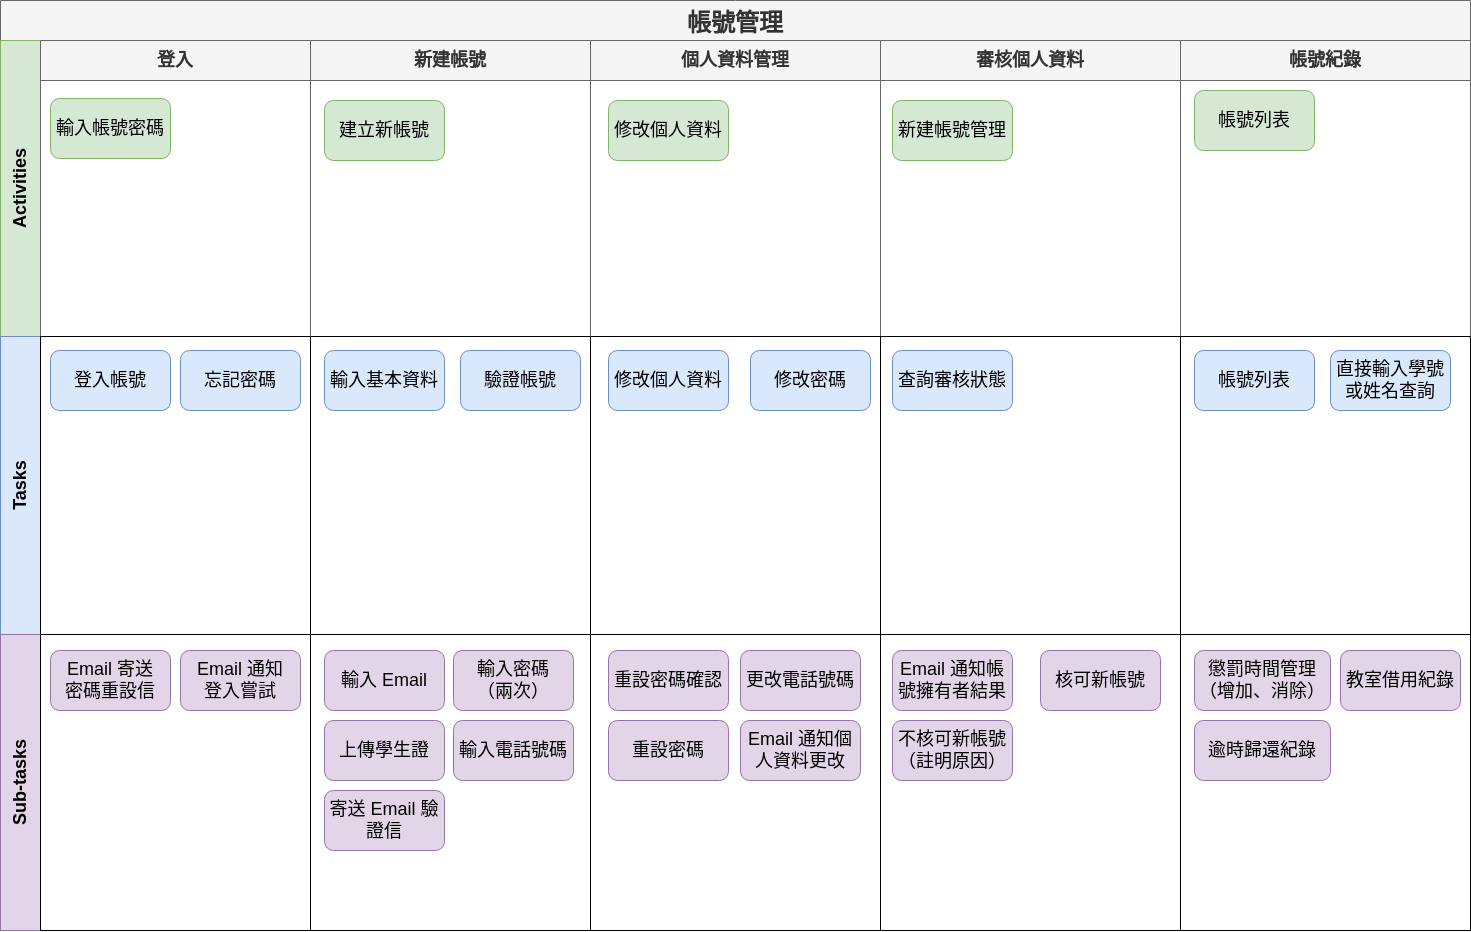
\includegraphics[height=0.45\textheight]{UserStoryMap-AccountManagement.png}
\end{center}

\begin{center}
	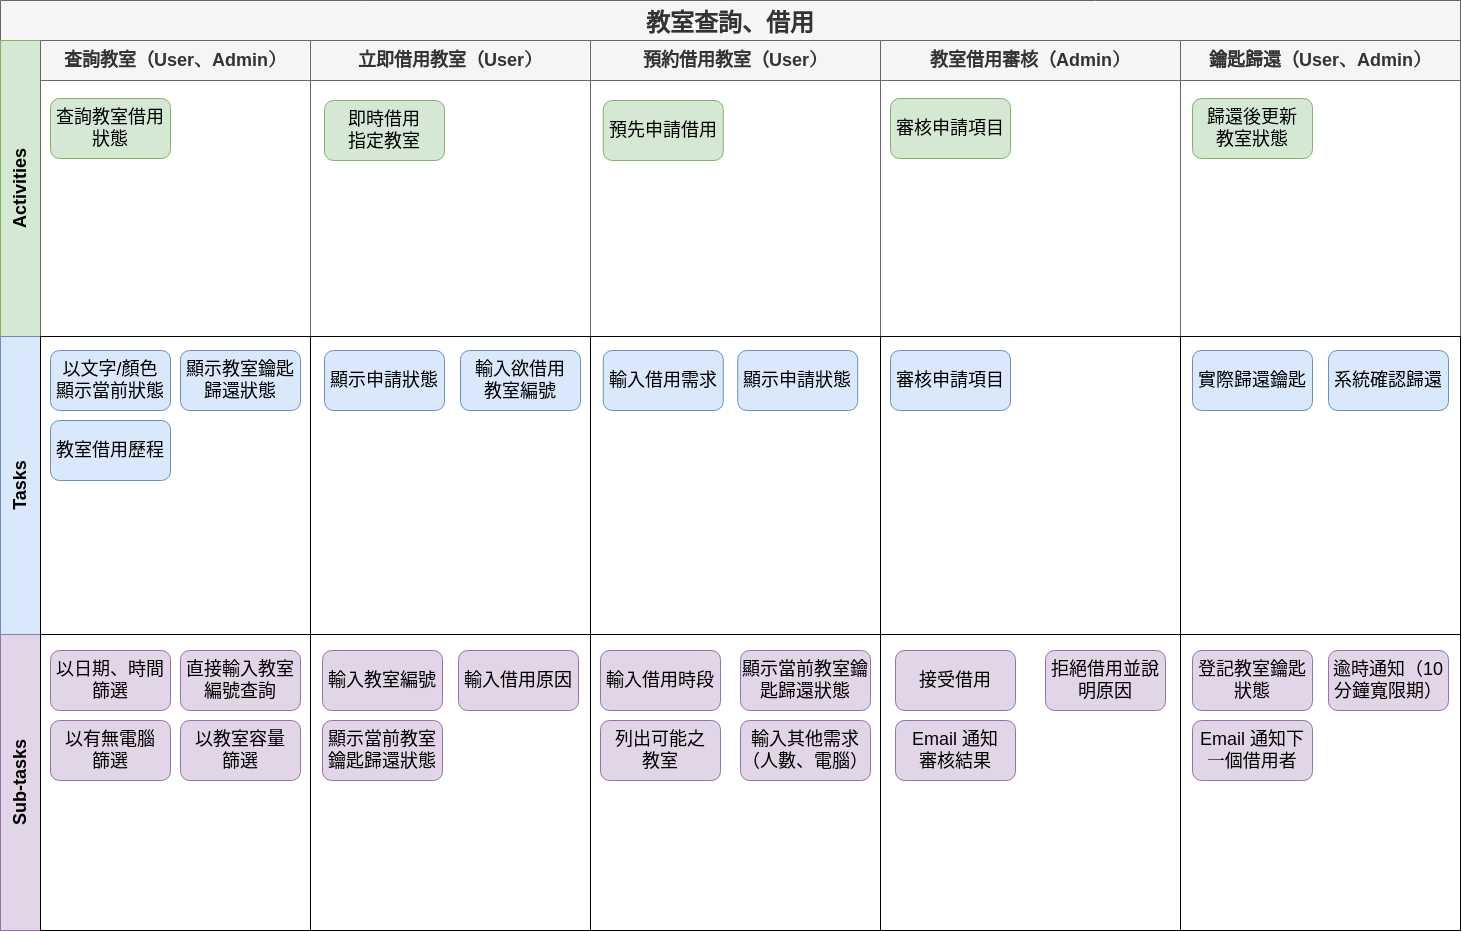
\includegraphics[height=0.45\textheight]{UserStoryMap-ClassroomBorrowing.png}
\end{center}
\newpage

\begin{table}[H]
	\begin{tabular}{| m{13cm} |}
		\hline
		代號:CPB-AM-LOG-01	帳號登入         \\ \hline
		故事:做為一個使用者,我可以在登入頁面輸入帳號與密碼登入。 \\	\hline
		註記:
		\begin{itemize}
			\item 可考慮在密碼變更後立即登出帳號
		\end{itemize}          \\ \hline
		測試方法:
		\begin{itemize}
			\item 輸入無效帳號
			\item 輸入有較帳號及錯誤密碼
			\item 在密碼變更後登入
		\end{itemize}
		\\	\hline
	\end{tabular}
\end{table}

\begin{table}[H]
	\begin{tabular}{| m{13cm} |}
		\hline
		代號:CPB-AM-REG-01	帳號註冊                         \\ \hline
		故事:做為一個使用者,我可以在登入頁面選擇註冊新帳號,並輸入電子郵件、學號與密碼進行註冊。 \\	\hline
		註記:
		\begin{itemize}
			\item 無
		\end{itemize}                                \\ \hline
		測試方法:
		\begin{itemize}
			\item 輸入無效電子郵件
			\item 兩次輸入密碼時輸入不一致
			\item 輸入已被註冊之帳號
		\end{itemize}
		\\	\hline
	\end{tabular}
\end{table}

\begin{table}[H]
	\begin{tabular}{| m{13cm} |}
		\hline
		代號:CPB-AM-PIN-01	使用者資料變更                    \\ \hline
		故事:做為一個使用者,我可以在個人資料頁面加入或修改個人帳號資料、或進行密碼變更作業。 \\	\hline
		註記:
		\begin{itemize}
			\item
		\end{itemize}                              \\ \hline
		測試方法:
		\begin{itemize}
			\item 輸入格式錯誤電話號碼
			\item 使用忘記密碼功能,並於電子郵件中的連結進行變更作業
		\end{itemize}
		\\	\hline
	\end{tabular}
\end{table}

\begin{table}[H]
	\begin{tabular}{| m{13cm} |}
		\hline
		代號:CPB-AM-PIV-01	帳號申請檢核                                \\ \hline
		故事:做為一個管理者,我可以在帳號管理頁面檢視新註冊帳號的資料,並根據郵件審核結果等因素認可或否決帳號申請。 \\	\hline
		註記:
		\begin{itemize}
			\item 管理者必須附上否決原因
		\end{itemize}                                       \\ \hline
		測試方法:
		\begin{itemize}
			\item 新增一個電子郵件認證通過的帳號
			\item 新增一個電子郵件認證未通過的帳號
		\end{itemize}
		\\	\hline
	\end{tabular}
\end{table}

\begin{table}[H]
	\begin{tabular}{| m{13cm} |}
		\hline
		代號:CPB-AM-AR-01	使用者紀錄與違規懲罰                       \\ \hline
		故事:做為一個管理者,我可以在帳號管理頁面檢視所有帳號的借閱紀錄,並對違反規定的使用者進行懲罰。 \\	\hline
		註記:
		\begin{itemize}
			\item 管理者可附上懲罰原因
		\end{itemize}                                  \\ \hline
		測試方法:
		\begin{itemize}
			\item 對一個帳號新增懲罰時數
			\item 對一個帳號減少懲罰時數
			\item 檢視一個帳號的紀錄
		\end{itemize}
		\\	\hline
	\end{tabular}
\end{table}

\begin{table}[H]
	\begin{tabular}{| m{13cm} |}
		\hline
		代號:CPB-CBI-LOG-01	教室狀態查詢      \\ \hline
		故事:做為一個使用者,我可以在教室查詢頁面檢視教室的狀態。 \\	\hline
		註記:
		\begin{itemize}
			\item 可用不同裝置查詢比較
		\end{itemize}               \\ \hline
		測試方法:
		\begin{itemize}
			\item 對一個教室進行借用,並檢視狀態
			\item 對一個教室進行預約,並檢視狀態
			\item 以時間篩選教室類型
			\item 以容量篩選教室類型
			\item 以教室編號進行查詢
			\item 以有無電腦進行查詢
		\end{itemize}
		\\	\hline
	\end{tabular}
\end{table}

\begin{table}[H]
	\begin{tabular}{| m{13cm} |}
		\hline
		代號:CPB-CBI-REG-01	教室直接借用          \\ \hline
		故事:做為一個使用者,我可以輸入教室編號或直接在查詢介面進行借用。 \\	\hline
		註記:
		\begin{itemize}
			\item 借用者必須輸入借用原因
		\end{itemize}                  \\ \hline
		測試方法:
		\begin{itemize}
			\item 對一個教室進行借用
			\item 兩隻帳號同時對一個教室進行借用
			\item 在懲罰未結束時進行借用
			\item 在以借用教室時進行借用
		\end{itemize}
		\\	\hline
	\end{tabular}
\end{table}

\begin{table}[H]
	\begin{tabular}{| m{13cm} |}
		\hline
		代號:CPB-CBI-REG-02	教室預約          \\ \hline
		故事:做為一個使用者,我可以輸入所需時段及器材等需求進行預約。 \\	\hline
		註記:
		\begin{itemize}
			\item 無
		\end{itemize}                  \\ \hline
		測試方法:
		\begin{itemize}
			\item 對一個教室進行借用
			\item 兩隻帳號同時對一個教室進行借用
			\item 在懲罰未結束時進行借用
			\item 在以借用教室時進行借用
		\end{itemize}
		\\	\hline
	\end{tabular}
\end{table}

\begin{table}[H]
	\begin{tabular}{| m{13cm} |}
		\hline
		代號:CPB-CBI-BOR-03	預約審核       \\ \hline
		故事:做為一個管理者,我可以檢視並審核所有教室借用預約。 \\	\hline
		註記:
		\begin{itemize}
			\item 須註明否決理由
		\end{itemize}               \\ \hline
		測試方法:
		\begin{itemize}
			\item 對一個預約進行核可
			\item 對一個預約進行否決
			\item 傳送審核結果至Email
		\end{itemize}
		\\	\hline
	\end{tabular}
\end{table}

\begin{table}[H]
	\begin{tabular}{| m{13cm} |}
		\hline
		代號:CPB-CBI-KR-01	鑰匙歸還登記                                      \\ \hline
		故事:做為一個管理者,我可以在接受使用者歸還的鑰匙後改變教室狀態、對逾期的使用者進行通知或寄送EMAIL給下一個使用者。 \\	\hline
		註記:
		\begin{itemize}
			\item 無
		\end{itemize}                                               \\ \hline
		測試方法:
		\begin{itemize}
			\item 登記已歸還教室
			\item 對逾期使用者進行警告
			\item 傳送Email給下一個欲借用的使用者
		\end{itemize}
		\\	\hline
	\end{tabular}
\end{table}

\newpage

\section[操作概念(OPERATIONAL CONCEPTS)]{操作概念(Operational Concepts)}

\subsection{借用方}

目前的鑰匙借用流程需要使用者先到系辦確認空教室,在確認該時段無人之後登記借用,並於指定的時間再至系辦領取鑰匙。
借用完畢後,要到系辦歸還鑰匙並簽名確認,若借用結束時系辦已經關門,還要擇日到系辦簽名並取回抵押證件。
使用此平台可以有效減少實際往返系辦的次數。

\subsubsection{註冊帳號}

第一次使用時須先註冊帳號,註冊時需填寫姓名、學號、系級、電子郵件、密碼等資訊,並且需確認電子郵件。

\subsubsection{確認教室狀態}

登入後可於平台首頁確認每個教室的借用狀態,並且可點選教室名稱查看詳細資訊。

\subsubsection{借用教室鑰匙}

點擊教室後可以申請借用該教室,並且可選擇借用時段,等待管理者確認後於指定時間至系辦領取鑰匙。

\subsubsection{歸還鑰匙}

教室使用完後,先將鑰匙歸還至系辦再點選平台上的歸還鑰匙按鈕,系辦收到鑰匙後會發送 Email 通知使用者。

\subsection{管理方}

對於管理方而言,相較於傳統的紙本文件,以網頁的形式來查看、管理教室借用的紀錄等資訊,能更直觀的分配教室,並且能夠即時的得知教室借用的狀態。

\subsubsection{管理鑰匙借用}

在有人申請借用教室時,管理者可以透過平台操作是否同意借用。

\bigskip

在教室借用時間結束,確認實際歸還鑰匙後,可以透過平台確認鑰匙歸還情形。
若在寬限期內未歸還鑰匙,系統將會自動發送 Email 通知使用者,並予以懲罰。


\newpage

\section[功能需求(FUNCTIONAL REQUIREMENTS)]{功能需求(Functional Requirements)}
\begin{tabular}{|l|c|c|}
	\hline
	功能編號                      & 功能名稱   & 功能說明                        \\ \hline
	\multicolumn{3}{| c |}{Account Management(帳號管理)}                 \\ \hline
	CBP-AM-LOG-01             & 帳號登入   & 使用者/管理員可於登入介面登入帳號           \\ \hline
	CBP-AM-REG-01             & 帳號註冊   & 使用者可使用 Email 與自訂密碼進行註冊      \\ \hline
	CBP-AM-PIM-01             & 個人資料管理 & 使用者可更改密碼與電話號碼               \\ \hline
	\color{blue}CBP-AM-PIV-01 & 審核個人資料 & 管理員可根據 Email 認證結果核可/否決新辦帳號  \\ \hline
	\color{blue}CBP-AM-AR-01  & 帳號紀錄   & 管理員可根據學號/姓名等資訊查詢使用者使用紀錄     \\ \hline
	\multicolumn{3}{| c |}{Classroom Borrowing \& Inquiring(教室租借查詢)} \\ \hline
	CBP-CBI-LOG-01            & 教室查詢   & 使用者可查詢教室目前使用狀態              \\ \hline
	CBP-CBI-BOR-01            & 教室立即借用 & 使用者可輸入教室編號進行借用              \\ \hline
	CBP-CBI-BOR-02            & 教室預約借用 & 使用者可輸入時段及需求進行申請             \\ \hline
	\color{blue}CBP-CBI-BOR-3 & 預約審核   & 管理員可對預約進行審核                 \\ \hline
	\color{blue}CBP-CBI-KR-1  & 鑰匙歸還登記 & 管理員可變更教室狀態                  \\ \hline
\end{tabular}
\newpage

\section[非功能需求(NON-FUNCTIONAL REQUIREMENTS)]{非功能需求(Non-Functional Requirements)}
\begin{tabularx}{\textwidth}{|l|c|Y|}
	\hline
	功能編號       & 功能名稱  & 功能說明                                 \\ \hline
	CBP-NFR-01 & 延遲時間  & 狀態更新後延遲不超過一分鐘                        \\ \hline
	CBP-NFR-02 & 密碼安全  & 密碼皆以雜湊後之形式傳輸、儲存                      \\ \hline
	CBP-NFR-03 & 人性化介面 & 查詢教室以前端實作,避免過度換頁造成瀏覽困難(如 tronclass ) \\ \hline
	CBP-NFR-04 & 驗證帳號  & 註冊後需要經過驗證方可開始借用教室                    \\ \hline
\end{tabularx}
\newpage

\section[使用者介面分析(USER INTERFACE ANALYSIS)]{使用者介面分析(User Interface Analysis)}

\begin{minipage}{0.6\linewidth}
	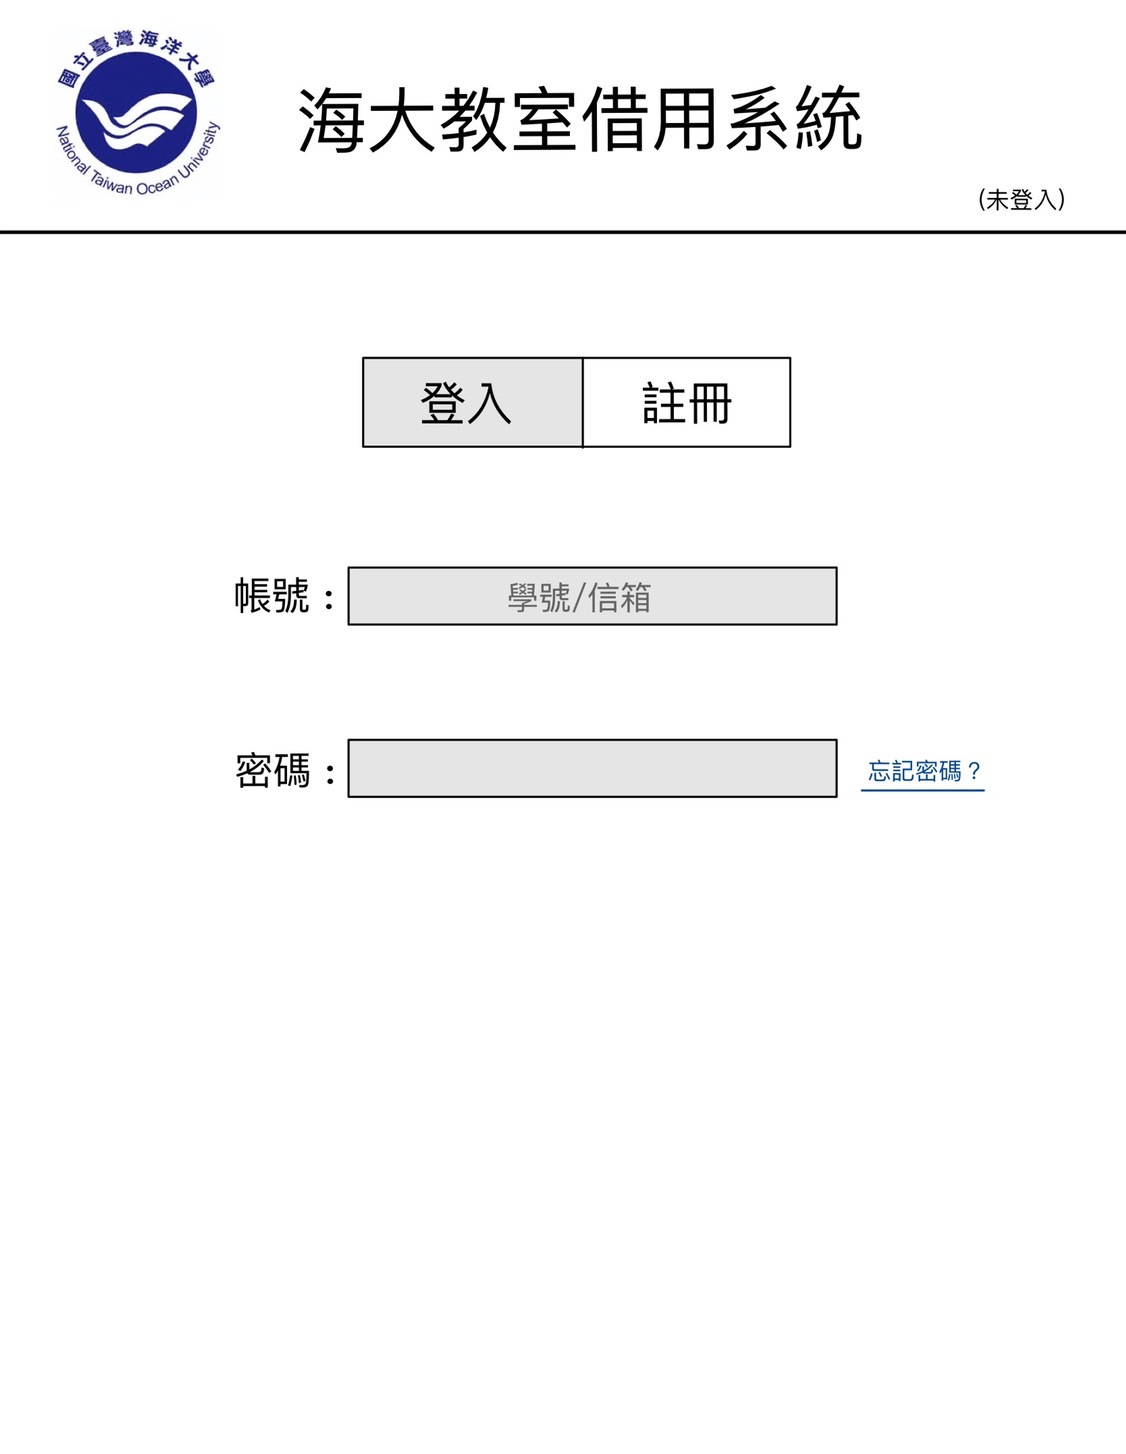
\includegraphics[height=0.4\textheight]{Log_In_GUI.jpg}
\end{minipage}
\begin{minipage}{0.4\linewidth}
	\subsection*{登入介面:}使用者可輸入學號/Email及密碼進行登入、或使用忘記密碼功能
\end{minipage}

\begin{minipage}{0.6\linewidth}
	\subsection*{註冊介面:}使用者可輸入學號、Email帳號並重複兩次自訂密碼註冊
\end{minipage}
\begin{minipage}{0.4\linewidth}
	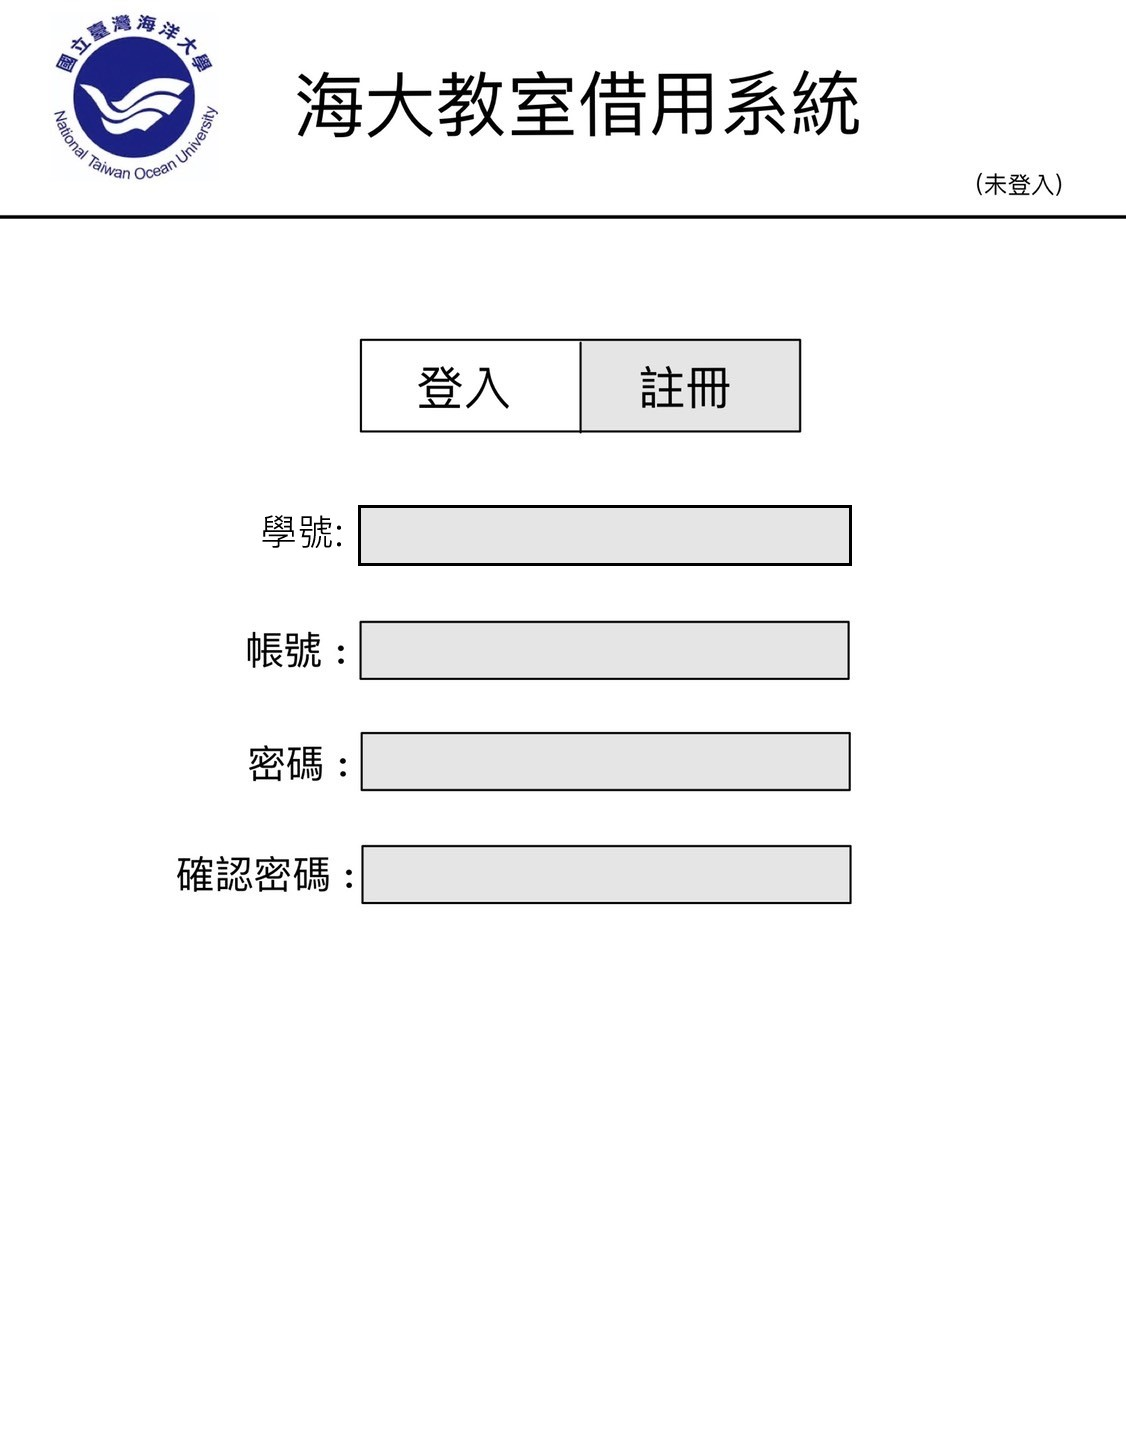
\includegraphics[height=0.4\textheight]{Regester_GUI.jpg}
\end{minipage}

\newpage
\subsection*{教室借用介面:}
\medskip
\begin{minipage}{0.6\linewidth}
	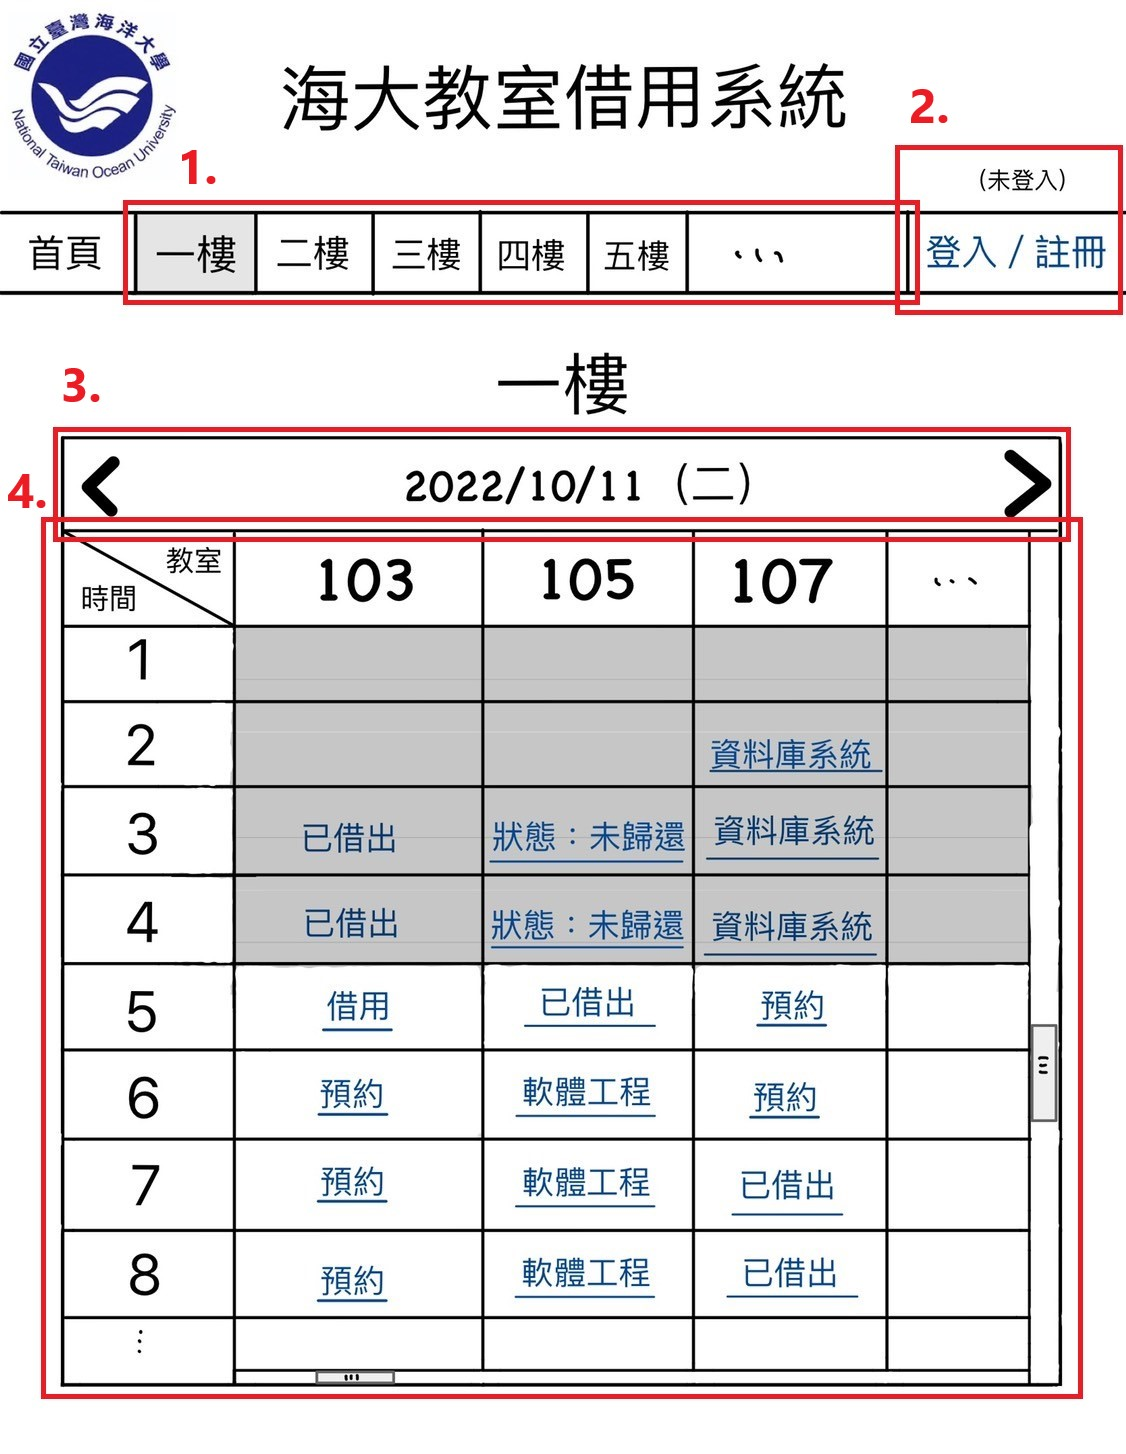
\includegraphics[height=0.4\textheight]{Borowing_GUI.jpg}
\end{minipage}
\begin{minipage}{0.4\linewidth}
	\subsubsection*{\textcolor{red}{1.}樓層選擇:}可選擇系館樓層
	\subsubsection*{\textcolor{red}{2.}登入狀態:}可按此登入、登出
	\subsubsection*{\textcolor{red}{3.}日期選擇:}可選擇欲借用之日期
	\subsubsection*{\textcolor{red}{4.}教室狀態:}直行為時間、橫列為教室,教室狀態有:已有固定課程、已經借用、尚未歸還鑰匙、可借用
\end{minipage}

\end{document}
